\documentclass[11pt]{article}

\usepackage[margin=1in]{geometry}
\usepackage{ifxetex}
\ifxetex
  % XeLaTeX (tectonic, lokal)
  \usepackage{fontspec}
  \setmainfont{lmroman10-regular.otf}[
    BoldFont=lmroman10-bold.otf,
    ItalicFont=lmroman10-italic.otf,
    BoldItalicFont=lmroman10-bolditalic.otf,
  ]
  \setsansfont{lmsans10-regular.otf}[
    BoldFont=lmsans10-bold.otf,
    ItalicFont=lmsans10-oblique.otf,
  ]
  \setmonofont{lmmono10-regular.otf}
\else
  % pdfLaTeX (Overleaf)
  \usepackage[T1]{fontenc}
  \usepackage[utf8]{inputenc}
  \usepackage{lmodern}
\fi
\usepackage[english]{babel}
\usepackage{amsmath,amssymb}
\usepackage{graphicx}
\usepackage{grffile}
\usepackage{float}
\usepackage{booktabs}
\usepackage{array}
\usepackage[authoryear,round]{natbib}
\usepackage{url}
\usepackage{hyperref}
\usepackage{caption}
\usepackage{setspace}
\usepackage{framed}
\usepackage{xcolor}

\setlength{\parindent}{0pt}
\setlength{\parskip}{0.8\baselineskip}
\emergencystretch=2em

\hypersetup{
    colorlinks=true,
    linkcolor=black,
    citecolor=blue!60!black,
    urlcolor=blue!60!black,
}

% --- kisaltmalar ---
\newcommand{\ltyirmi}{$<\!20\%$}
\newcommand{\fairs}{\textit{fairness\_salience}}
\newcommand{\disp}{\textit{disposable\_income\_buffer}}

% --- finding / verdict kutulari ---
\definecolor{shadecolor}{rgb}{0.96,0.96,0.96}
\newenvironment{findingbox}{%
    \begin{shaded}\noindent\textbf{FINDING.}\quad}{\end{shaded}}

\newcommand{\verdictbox}[1]{%
    \begin{center}
    \fbox{\parbox{0.92\linewidth}{\centering\textbf{#1}}}
    \end{center}}

\title{\textbf{LLMs Simulate the Description of a Culture, Not the Culture}\\[0.3em]
\large An Attempt to Reproduce Henrich's Cross-Cultural Ultimatum Game Finding with LLM Agents}

\author{Gökhan Geyik\\\textit{Empler AI}\\\texttt{gokhan@empler.ai}\\ORCID: \href{https://orcid.org/0009-0000-9028-1827}{0009-0000-9028-1827}}

\date{October 2026}

\begin{document}

\maketitle

\begin{abstract}
\noindent
Describing a cultural identity to a large language model (LLM) and using it in place of human participants is an increasingly common method in generative agent-based modeling (GABM). We test the validity of this method against one of the best-documented cross-cultural findings in behavioral economics: in the Ultimatum Game, WEIRD students frequently reject low offers (40--60\%), whereas in several small-scale societies with low market integration low offers are rarely rejected. Using three model families (Claude Haiku 4.5, Gemma-4-31b-it, GPT-OSS-120b), we ran a sequential investigation in which the hypotheses and analysis plan of every step were filed in writing before its data were collected. For the same identities, the same game and the same offers, the outcome changed fundamentally with nothing but the wording of the identity description. When a numeric ``fairness salience'' score was added to the description, following classical agent-based modeling practice (Study~1), models rejected 10\% offers only 3\% of the time; raising the score on the same card from 0.3 to 0.6 raised low-offer rejection across the three models from 5\% to 52\%. With the numbers removed (Study~2), a gap \emph{opposite} to Henrich's appeared: small-scale cards rejected 61\% of 10\% offers, WEIRD cards 6\% (same direction in all three models). This reversed gap, however, appeared only when the description contained value-laden phrases such as ``reciprocity, sharing, kin network''; when the identity was described only by age and occupation, or by a text stating community size and market integration factually, the gap between arms vanished (21\% vs.\ 24\%; 13\% vs.\ 9\%). No description produced the pattern Henrich observed. LLM agents steered by an identity description reflect how a culture is described rather than how its members behave; numeric and value-laden elements of the description can determine both the existence and the direction of a cross-cultural result.
\end{abstract}

\textbf{Keywords:} Ultimatum Game $\cdot$ large language models $\cdot$ generative agent-based modeling $\cdot$ cross-cultural behavior $\cdot$ WEIRD $\cdot$ persona simulation $\cdot$ prompt sensitivity $\cdot$ replication


\section{Introduction}

The Ultimatum Game \citep{guth1982} is a minimal bargaining situation: a proposer offers the responder a share of a 100-unit pot; if the responder accepts, both receive their shares, and if the responder rejects, both receive nothing. A self-interested responder should accept any positive offer, yet human participants routinely reject low offers. \citet{henrich2001}, in field experiments in 15 small-scale societies, showed that this behavior varies greatly across cultures: WEIRD (Western, Educated, Industrialized, Rich, Democratic) university students reject offers below 20\% of the pot 40--60\% of the time, while in several societies with low market integration low offers were almost never rejected: among the Machiguenga of the Peruvian Amazon only one offer was rejected although most offers were low, and among the Tsiman\'e none was. This is among the most cited pieces of evidence that fairness norms are not universal \citep{henrich2010}.

In recent years LLMs have been increasingly used as ``silicon'' stand-ins for human participants \citep{argyle2023,horton2023,aher2023,park2023}. For cross-cultural research the approach is especially attractive: telling an LLM ``you are a subsistence farmer in the Amazon'' costs a small fraction of fieldwork. Its core assumption is that a model steered by an identity description reflects the behavior of real people with that identity. Evidence that LLMs flatten and caricature identity groups \citep{cheng2023compost,wang2025misportray}, that their psychology resembles WEIRD populations \citep{atari2023which}, and that they are highly sensitive to meaningless changes in prompt formatting \citep{sclar2024quantifying} calls this assumption into question.

We attempt to reproduce Henrich's finding within a GABM framework with three model families. The study was initially designed as a single experiment. Its unexpected result was examined through a sequence of tests; the hypotheses and decision rules of each test were filed in writing after the result of the previous test was known but before its own data were collected (Section~\ref{sec:prereg}). We report this sequential process as it happened. The main claim rests on two direct manipulations: presenting the same identities with and without numeric attributes (Section~\ref{sec:numbers}), and describing the same identities in three different texts (Section~\ref{sec:wording}). The findings are:

\begin{enumerate}
\item \textbf{Numeric attributes set the outcome.} A ``fairness salience'' score added to the description largely determines the rejection rate. In the first experiment with these scores (Study~1) the models almost never rejected; a separate test shows this was largely due to the low scores on the cards.
\item \textbf{Value-laden words set the direction of the gap.} With the numbers removed (Study~2), a gap opposite to Henrich's appeared. It appears when the small-scale identity is described with phrases such as ``reciprocity, sharing, kin network'' and disappears when the same identity is described in plain or factual language.
\item \textbf{No description reproduces Henrich.} Even when community size and market integration, the explanatory variables in the human data, are described factually, the models do not produce the human pattern.
\end{enumerate}

These findings carry a concrete warning for GABM practitioners: the output of an LLM steered by an identity description is a function of how the researcher describes the group, not of the group's behavior.


\section{Related Work}

\subsection{The Ultimatum Game and cross-cultural variation}

Since \citet{guth1982} introduced the Ultimatum Game, thousands of experiments have examined the consistency and determinants of rejection behavior. The first wave, conducted with WEIRD samples, documented that offers below 20\% are routinely rejected and that the modal offer is 40--50\%. The simultaneous field experiments of \citet{henrich2001} in 15 small-scale societies showed that this picture was a misleading generalization: communities such as the Machiguenga were characterized by very low rejection rates, while others, such as the Lamalera (Indonesia), stood out with hyper-fair offers ($>$50\%).

\citet{henrich2010} placed these findings in a broader framework, noting that 96\% of samples in psychology come from countries that are home to only 12\% of the world's population. The ``WEIRD problem'' is among the most influential methodological critiques in modern behavioral economics and psychology. It also indicates why proposals such as GABM matter: ethical, financial and practical barriers make cross-cultural fieldwork difficult.

\subsection{LLMs as silicon subjects}

The idea of LLMs as stand-ins for behavioral subjects emerged from several research programs. \citet{binz2023} administered classic cognitive psychology tasks to GPT-3 and reported patterns qualitatively similar to, but not identical with, human results. \citet{horton2023} argued, within the ``Homo silicus'' framework, that LLMs can be used in simulations of economic agents and showed that several classic experimental economics results can be reproduced qualitatively. \citet{argyle2023} showed that GPT-3, with appropriate demographic conditioning, can mimic the response distributions of US survey subgroups.

\citet{aher2023} extended this agenda with ``Turing experiments'', testing how well LLMs reproduce human results in classic paradigms such as the Ultimatum Game, garden-path sentences, the Milgram shock experiment and the wisdom of crowds; the study did not compare cultural profiles. \citet{park2023} laid the architectural foundation of GABM with generative agents that produce social dynamics in a simulated town. \citet{mei2024} ran a ``behavioral Turing test'' across behavioral games and personality measures and reported that ChatGPT-4 falls within the distribution of human participants but is more cooperative and altruistic than the average human. This is directionally consistent with our Study~1 and with the WEIRD arm of Study~2, but the small-scale arm of Study~2 shows the opposite.

\subsection{Persona simulation and group representation}

\citet{cheng2023compost} showed that LLM simulations tend to render personas as exaggerated caricatures rather than multidimensional individuals and proposed a framework to measure this. \citet{wang2025misportray} showed analytically and empirically that LLMs replacing human participants both misportray identity groups and flatten within-group diversity. \citet{atari2023which} reported that LLM responses to psychological measures most resemble WEIRD populations and that the resemblance declines quickly with cultural distance from them. We add a pre-specified test in a behavioral decision paradigm, against a direct human anchor (Henrich's field data).

\subsection{Prompt sensitivity}

The sensitivity of LLM outputs to prompt wording is well documented. \citet{sclar2024quantifying} showed that meaning-preserving formatting changes can shift performance of open models by up to 76 points and that the sensitivity persists with model size and instruction tuning. For persona simulation, \citet{hu2024persona} reported that persona variables supplied in the prompt give modest but significant gains on subjective annotation tasks, larger where the variables are strongly related to human responses. We carry this literature into a behavioral decision paradigm. Here the description changes do not preserve meaning; each emphasizes a different, defensible aspect of the same identity, and this difference in emphasis can reverse a cross-cultural result measured against a human anchor.

\subsection{Entitlement and allocation}

In human experiments, having earned the resource to be divided changes allocation markedly. Proposers who earn their role through a quiz offer less \citep{hoffman1994}; dictators who earn the money give almost nothing \citep{cherry2002}; when the recipient earned it, dictators may leave more than half \citep{oxoby2008}. In the standard Ultimatum Game the pot is handed out by the experimenter as a windfall.


\section{General Method}

\subsection{Paradigm and cultural arms}

All experiments use the one-shot anonymous Ultimatum Game. The pot is 100 units; offer levels are 10, 20, 30, 40 and 50\%. The proposer agent delivers the offer assigned to it and predicts what the responder will do; the responder agent accepts or rejects. Both agents write a two-to-three-sentence justification.

Each agent receives a short identity description, which we call a \emph{card}. Cultural arms are presented as \emph{identity}, never as behavioral instruction. Below is the \emph{value-laden} description used in Studies~1 and~2; Section~\ref{sec:wording} tests two alternatives. \textbf{WEIRD card:} aged 19--24, a university student (economics, psychology, computer science, biology, history, business, sociology or statistics); ``supported by family or loans, low subsistence risk''; ``moderate, mostly classmates and friends''; formal market experience; high institutional trust. \textbf{Small-scale card:} aged 22--45; subsistence farming, small-scale fishing, herding, craft trade or seasonal labor; ``buffered by kinship network, no formal wage''; ``dense kin network, daily face-to-face community''; ``non-market reciprocity, sharing, barter''; low institutional trust. Card texts pass an automatic linter that bans terms such as ``reject'', ``accept'', ``fair'', ``fairness'', ``rational'', ``utility'' and ``ultimatum game''.

\subsection{Models}

We use three model families from three providers (Table~\ref{tab:models}).

\begin{table}[H]
\centering
\caption{Models used in the study.}
\label{tab:models}
\begin{tabular}{llll}
\toprule
Role & OpenRouter slug & Provider & Access \\
\midrule
Primary / sweep base & \texttt{anthropic/claude-haiku-4.5} & Anthropic & closed API \\
Secondary & \texttt{google/gemma-4-31b-it} & Google & open weights \\
Tertiary & \texttt{openai/gpt-oss-120b} & OpenAI & open weights \\
\bottomrule
\end{tabular}
\end{table}

All calls use temperature $T = 0.4$, which keeps response variance low while preserving sensitivity to manipulations. Every response is returned as structured output against a predefined JSON schema; no response is parsed with regular expressions.

\subsection{Agent prompts and output schemas}

\textbf{System prompt (both roles):}

\begin{quote}
\itshape
``You are a participant in a one-shot anonymous behavioral experiment. You will not meet the other participant again. Reason from your identity. Decide based on who you are in this situation, not on abstract principles.''
\end{quote}

\textbf{Game mechanics (responder version, with \{offer\} and \{keep\} filled in):}

\begin{quote}
\itshape
``There is a pot of 100 units. The other person has been asked to propose a split. They offered you \{offer\} units, which means they would keep \{keep\} units. If you accept, you receive \{offer\} and they receive \{keep\}. If you decline, both of you receive 0. This is a one-time decision --- there are no further rounds.''
\end{quote}

The terms ``Ultimatum Game'', ``rational'', ``utility'', ``economic theory'' and ``fair offer'' appear nowhere in the prompt chain. Outputs follow these schemas:

\begin{itemize}
\item \textbf{Proposer:} \texttt{\{offer: int, expected\_responder\_action: "accept"|"decline", reasoning: str\}}
\item \textbf{Responder:} \texttt{\{action: "accept"|"decline", reasoning: str\}}
\end{itemize}

\subsection{Pre-registration procedure}\label{sec:prereg}

For every experiment, hypotheses, decision rules and the analysis plan were written to a separate file before the first API call. In this paper we use ``pre-registered'' only in this sense: these files were not uploaded to a public, time-stamped registry such as OSF or AsPredicted, and their time of writing cannot be independently verified. All files, including dated notes added later, are in the replication package, so readers can compare each test's decision rule with its results. Before each main run a small pilot (``smoke'') run was executed and its reasoning texts were read for design flaws; pilot data were excluded from all analyses. Every change after a pilot was added to the pre-registration as a dated amendment with its rationale. Occasional empty responses from some providers (\texttt{\{"action": -1\}}) were not coded as decisions; they were re-requested and counted. All calls are logged with time stamps and session identifiers.

\subsection{Coding of justification texts}

Responder justifications were coded by two \emph{decision models} from providers different from all generating models: TypeSafe Jev~1.13 \citep{typesafe2026jev} and Respan Span-01 \citep{respan2026span}. These models do not generate text; they return the probability of ``yes'' for a defined yes/no question. The codebook has seven themes: \emph{material need/survival}, \emph{kin/community}, \emph{game theory/expected value}, \emph{refusal as self-harm}, \emph{fairness judgement}, \emph{equal-split norm} and \emph{anonymity/one-shot interaction}. Each text is coded on its own, to avoid order and context effects; the coder receives only the justification text, not the card, prompt, arm or offer. Span-01 is deterministic; Jev has small repeat variance (SD $\approx 0.011$ across repeats), so each text is the mean of three calls. A theme counts as present at probability $\geq 0.5$. Arm separability is measured as the accuracy of a leave-one-out (LOO) linear classifier predicting the arm from the seven theme probabilities.


\section{Study 1: cards with numeric attributes}\label{sec:study1}

\subsection{Design and hypotheses}

In Study~1, two numeric attributes were added below each card, to allow comparison with a rule-based baseline from classical agent-based modeling and to create heterogeneity between agents:

\begin{quote}
\ttfamily\small
INTERNAL NUMERIC ATTRIBUTES (for your own reflection, not instructions):\\
- fairness\_salience (0-1 scale): 0.2\\
- disposable\_income\_buffer: 28.1
\end{quote}

\fairs{} was drawn from $[0.4,\,0.8]$ for WEIRD cards and $[0.2,\,0.6]$ for small-scale cards; \disp{} from $[200,\,5\,000]$ and $[20,\,800]$ respectively, via a Pareto($\alpha = 2$) distribution. This distribution concentrates values at the lower end of each range: the realized median \fairs{} is 0.40 for WEIRD cards and 0.20 for small-scale cards. The design is 3 models $\times$ 2 arms $\times$ 5 offers $\times$ 50 pairs (1\,500 pairs, 3\,000 calls; $T = 0.4$).

Pre-registered hypotheses (\ltyirmi{} = offer of 10\%): \textbf{H1} WEIRD rejection rate $\in [0.30,\,0.70]$; \textbf{H2} small-scale rejection rate $\in [0.00,\,0.30]$; \textbf{H3} WEIRD $-$ small-scale gap $\geq 0.15$, $\chi^2$ $p_{\text{Bonf}} < 0.01$ ($k = 5$) and Cohen $h \geq 0.3$; \textbf{H4} rejection decreases monotonically with the offer in each arm (Spearman $\rho < -0.9$); \textbf{H5} no model's rate deviates from the three-model mean by more than 0.15 in any cell. Decision rule: H1 $\wedge$ H2 $\wedge$ H3 $\Rightarrow$ Henrich replicated. The WEIRD band follows the commonly reported 40--60\% rejection of offers below 20\% in student samples. The small-scale band (0.05--0.25 as anchor, widened to 0.00--0.30 for H2) is our pre-specified composite for societies in which low offers were rarely rejected; rejection behavior in Henrich's sample is heterogeneous across societies, and the band is not a statistic reported by \citet{henrich2001}.

\subsection{Results}

Only 14 rejections occurred in 1\,500 pairs (0.9\%). At a 10\% offer the rejection rate was 0.027 in the WEIRD arm and 0.040 in the small-scale arm (Table~\ref{tab:rejection}). H1 and H3 failed and the pre-registered decision is negative (Table~\ref{tab:gate}). The result did not change under two additional card wordings and two additional prompt wordings (2\,000 pairs, 2 rejections), two additional temperatures ($T = 0.0$ and $1.0$; 894 calls, rejection $\leq 0.9\%$) or a strengthened system prompt forcing the model to ``become'' the identity (150 calls, 150 acceptances). All of these robustness checks used cards with numeric attributes; as Section~\ref{sec:numbers} shows, what they show to be stable is largely the result produced by those numbers.

\begin{table}[H]
\centering
\caption{Pooled rejection rates ($N = 150$ per cell, three models).}
\label{tab:rejection}
\begin{tabular}{lrrrrr}
\toprule
Arm & 10\% & 20\% & 30\% & 40\% & 50\% \\
\midrule
WEIRD       & 0.027 & 0.013 & 0.000 & 0.000 & 0.000 \\
Small-scale & 0.040 & 0.007 & 0.007 & 0.000 & 0.000 \\
\bottomrule
\end{tabular}
\end{table}

\begin{figure}[H]
\centering
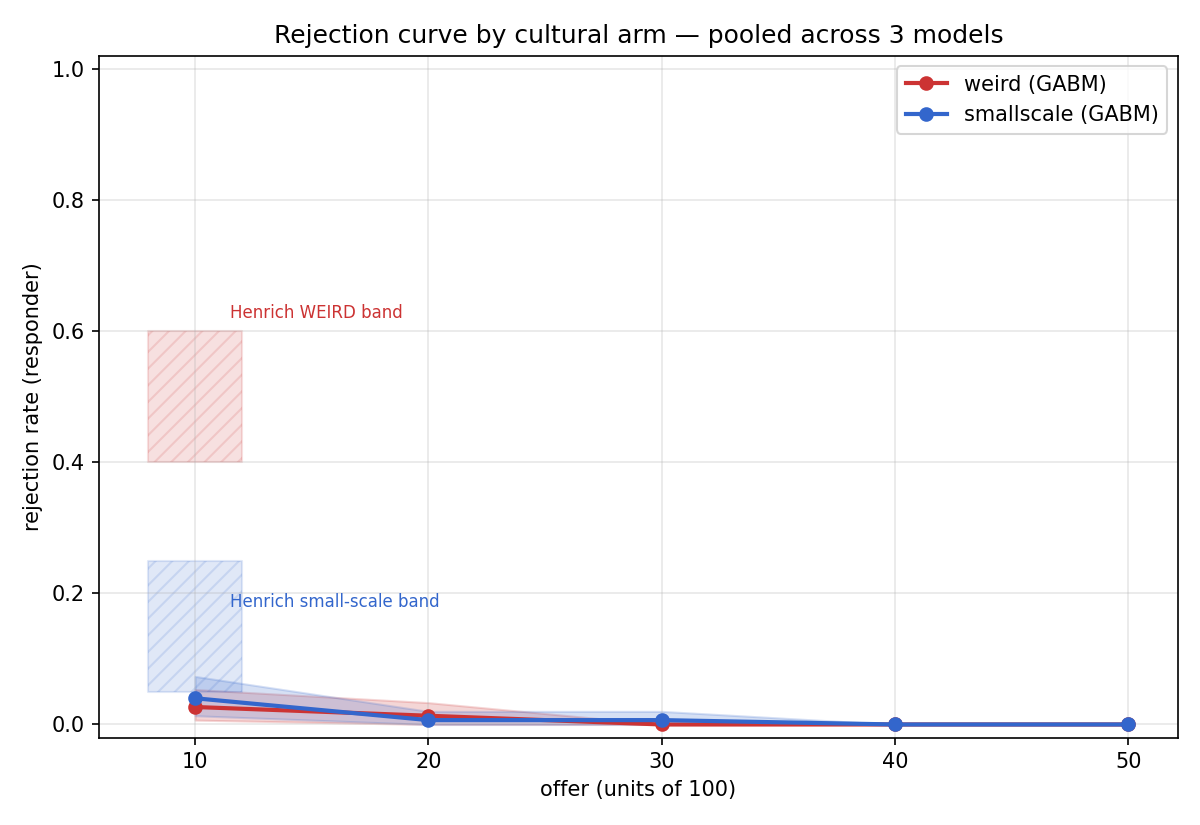
\includegraphics[width=0.85\linewidth]{figs/fig1.png}
\caption{Study~1 rejection rates by offer for the WEIRD and small-scale arms, with Henrich's anchor bands. All observed curves collapse toward zero; neither arm approaches Henrich's ranges.}
\label{fig:rejection}
\end{figure}

\begin{table}[H]
\centering
\caption{Study~1 pre-registered baseline gate.}
\label{tab:gate}
\begin{tabular}{llrl}
\toprule
Criterion & Threshold & Observed & Result \\
\midrule
H1 WEIRD \ltyirmi{}         & $\in [0.30,\, 0.70]$ & 0.027   & \textbf{FAIL} \\
H2 Small-scale \ltyirmi{}   & $\in [0.00,\, 0.30]$ & 0.040   & Pass \\
H3 gap $\geq 0.15$          & $\geq 0.15$          & $-0.013$ & \textbf{FAIL} (wrong direction) \\
H3 $p < 0.01$ Bonf.         & $p_{\text{Bonf}} < 0.01$ & 1.000 & \textbf{FAIL} \\
H3 Cohen $h \geq 0.3$       & $\geq 0.3$           & $-0.075$ & \textbf{FAIL} \\
H4 Spearman $\rho$ WEIRD    & $\rho < -0.9$        & $-0.894$ & Just below threshold \\
H4 Spearman $\rho$ Small    & $\rho < -0.9$        & $-0.949$ & Pass \\
H5 cross-model $\leq 0.15$  & $\leq 0.15$          & 0.080   & Pass \\
\bottomrule
\end{tabular}
\end{table}

\verdictbox{STUDY 1 PRE-REGISTERED DECISION: NEGATIVE --- no Henrich gap; the LLMs almost never rejected.}

The same models in the proposer role, however, predicted that low offers would be rejected: at a 10\% offer, 79\% of WEIRD and 45\% of small-scale proposers expected rejection. The models ``know'' that people reject low offers but do not behave that way as responders. The coded responder justifications are culturally distinguishable (arm predicted from seven themes: Jev 83\%, Span-01 84\%; $n = 1\,500$): small-scale justifications invoke kin and need, WEIRD justifications invoke expected-value reasoning. Yet the decision is ``accept'' in both arms. This is Study~1's open question: why do culturally distinct justifications arrive at the same decision?


\section{The effect of numeric attributes}\label{sec:numbers}

About 30\% of Study~1 responder justifications mention the numeric attributes by name (e.g., ``my low fairness salience (0.2)''). To measure their effect directly we ran a pre-registered test in which the same identity cards were shown in three ways: with the numeric block \emph{hidden}, with the \emph{same} low values for both arms (\fairs{} $= 0.3$, \disp{} $= 300$), and with the \emph{same} high values for both arms (\fairs{} $= 0.6$, \disp{} $= 300$). This factor was crossed with the source of the pot (windfall, jointly earned, placebo; see Appendix~\ref{sec:entitle}) and the frame (game text or disguised story; see Appendix~\ref{sec:disguise}). Each card saw all 18 conditions: 3 models $\times$ 2 arms $\times$ 2 offers (10\%, 20\%) $\times$ 50 cards $\times$ 18 conditions = 10\,800 calls, of which 10\,799 were valid.

\begin{figure}[H]
\centering
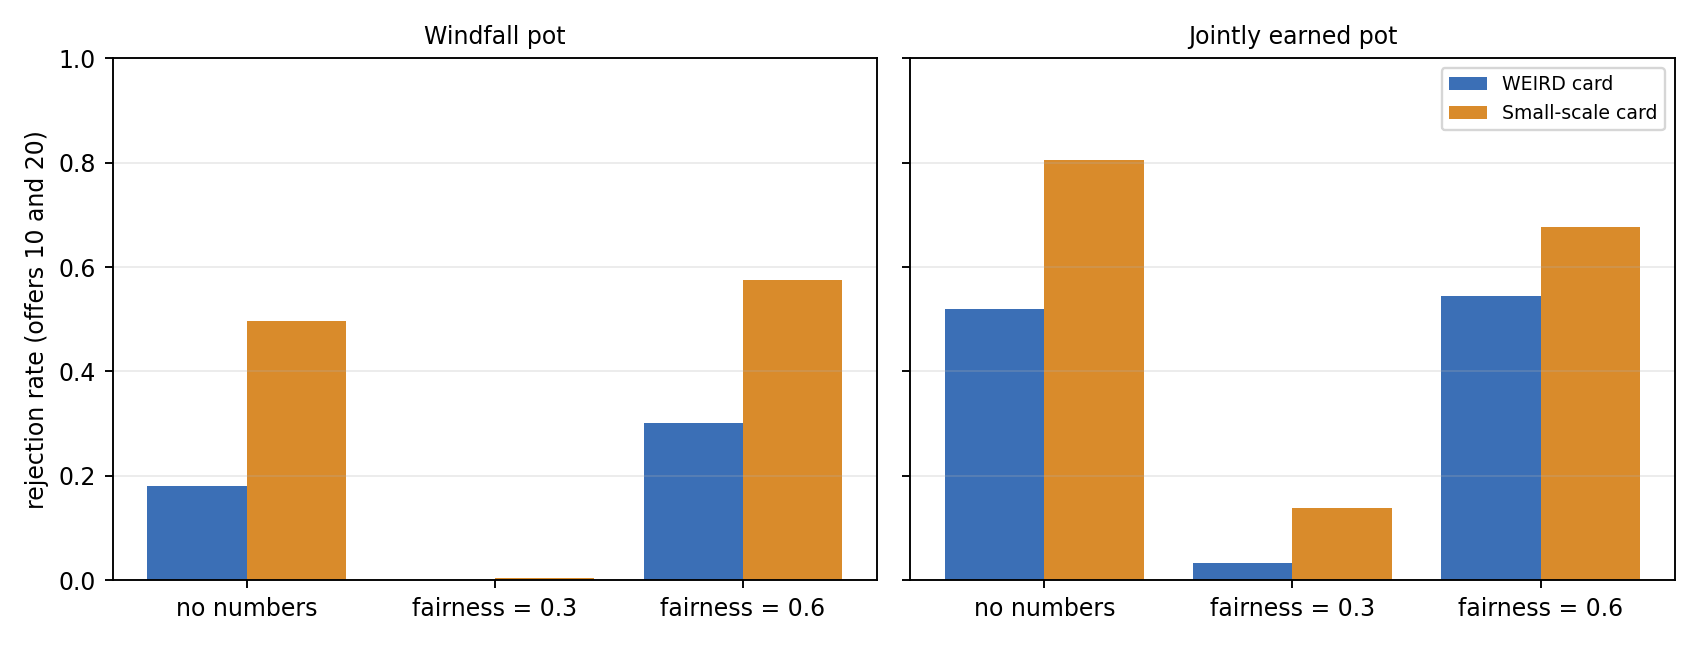
\includegraphics[width=0.95\linewidth]{figs/fig15_numbers.png}
\caption{Effect of numeric attributes: rejection rate at low offers (10\% and 20\%), three models and both frames pooled. Same identity cards; only the numeric block changes. With a fairness score of 0.3 there is almost no rejection; with 0.6, and with no numbers, rejection is high. With the numbers equalized or removed, small-scale cards reject more than WEIRD cards.}
\label{fig:numbers}
\end{figure}

\textbf{The number sets the decision.} In the pre-specified primary comparison (earned pot, Haiku and Gemma, both arms and frames), raising the fairness score on the same card from 0.3 to 0.6 raised low-offer rejection from \textbf{12.5\% to 80.5\%} (544 cards switched from accept to reject, none in the other direction; McNemar $p < 10^{-160}$). The effect is also present with a windfall pot: across the three models, rejection is 0--0.5\% at a score of 0.3 and 30\% (WEIRD) and 58\% (small-scale) at 0.6 (Figure~\ref{fig:numbers}). The most extreme case is Gemma: with an earned pot, WEIRD cards reject 2.5\% of the time at a score of 0.3 and 96.5\% at 0.6.

\textbf{Explaining Study~1.} In Study~1 the fairness scores were concentrated at the low end of their ranges (medians 0.40 and 0.20). The models read these low values as ``I don't care much about fairness'' and accepted. Of the 11 rare Study~1 cards with a score of 0.55 or higher, 8 rejected the low offer. Study~1's ``LLMs do not reject'' result is therefore largely produced by the numbers the design wrote onto the cards.

\textbf{With the numbers equalized, the arm gap reverses.} In the entitlement test, run earlier in chronological order (Appendix~\ref{sec:entitle}; with numeric cards), WEIRD cards rejected more often when the pot was earned (at low offers, 19\% vs.\ 8\% in the game frame and 48\% vs.\ 17\% in the story frame), which could have been read as a Henrich-direction gap. With the numbers equalized this gap vanished and reversed: with an earned pot, Haiku and Gemma pooled, small-scale cards rejected 100\% and WEIRD cards 74\% with the numbers hidden (gap $-0.26$, Fisher $p < 10^{-33}$), and the gap was $-0.11$ with the numbers equal ($p < 10^{-4}$). Because the pre-written decision rule only tested a Henrich-direction gap, it classified this result as ``no identity effect''; we recorded the strong reverse-direction gap as a separate note in the pre-registration and then tested it as a pre-registered hypothesis in Study~2. Its source is examined in Section~\ref{sec:wording}.


\section{Study 2: cards without numbers}\label{sec:study2}

\subsection{Design and hypotheses}

Study~2 repeats the design of Study~1 exactly, except that the numeric block is removed from the cards. The same identity cards are used for all three models. The design is 3 models $\times$ 2 arms $\times$ 5 offers $\times$ 50 pairs (1\,500 pairs, 3\,000 calls). H1--H5 are taken unchanged from Study~1. Two hypotheses were added before data collection: \textbf{H-R} (reversed gap): the small-scale $-$ WEIRD rejection gap at a 10\% offer is $\geq 0.15$, with $p_{\text{Bonf}} < 0.01$ and $|h| \geq 0.3$; \textbf{H-S1}: the rejection rate at a 10\% offer is at least 0.10 higher in Study~2 than in Study~1 (Fisher $p < 0.01$).

\subsection{Results}

\begin{table}[H]
\centering
\caption{Study~2 (no numbers): rejection rate by offer. Study~1 (numeric cards) in parentheses. Henrich's human anchors for \ltyirmi{}: WEIRD 0.40--0.60, small-scale 0.05--0.25.}
\label{tab:study2}
\begin{tabular}{llrrrrr}
\toprule
Model & Arm & 10\% & 20\% & 30\% & 40\% & 50\% \\
\midrule
All three & WEIRD       & 0.06 (0.03) & 0.00 (0.01) & 0.01 (0.00) & 0.00 & 0.00 \\
          & Small-scale & \textbf{0.61} (0.04) & 0.43 (0.01) & 0.39 (0.01) & 0.13 & 0.00 \\
\midrule
Gemma-4-31b-it   & WEIRD       & 0.18 & 0.00 & 0.00 & 0.00 & 0.00 \\
                 & Small-scale & \textbf{1.00} & 0.94 & 0.74 & 0.18 & 0.00 \\
GPT-OSS-120b     & WEIRD       & 0.00 & 0.00 & 0.02 & 0.00 & 0.00 \\
                 & Small-scale & \textbf{0.54} & 0.36 & 0.42 & 0.20 & 0.00 \\
Claude Haiku 4.5 & WEIRD       & 0.00 & 0.00 & 0.00 & 0.00 & 0.00 \\
                 & Small-scale & \textbf{0.28} & 0.00 & 0.00 & 0.00 & 0.00 \\
\bottomrule
\end{tabular}
\end{table}

\begin{figure}[H]
\centering
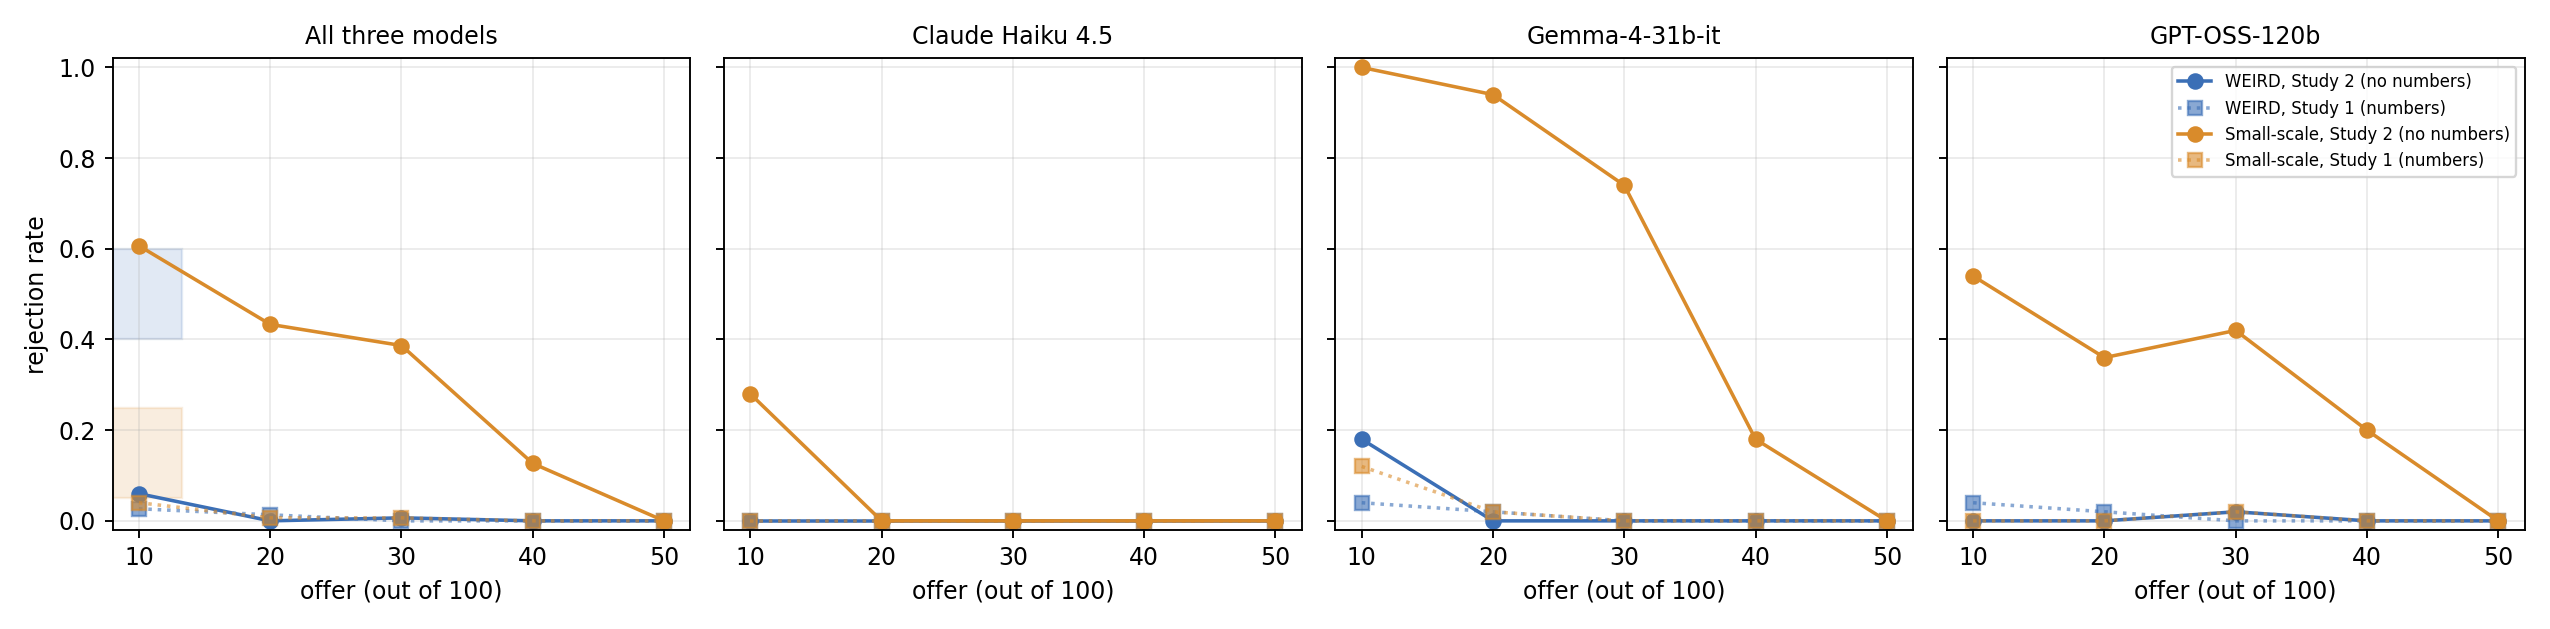
\includegraphics[width=\linewidth]{figs/fig16_study2.png}
\caption{Rejection curves for Study~2 (solid, no numbers) and Study~1 (dotted, numeric cards). Shaded areas in the left panel are Henrich's \ltyirmi{} human anchors (blue WEIRD, orange small-scale). Without numbers, small-scale cards rise into and beyond the human WEIRD range while WEIRD cards stay at zero.}
\label{fig:study2}
\end{figure}

At a 10\% offer, small-scale cards rejected \textbf{61\%} and WEIRD cards \textbf{6\%} of the time (Table~\ref{tab:study2}, Figure~\ref{fig:study2}): a small-scale $-$ WEIRD gap of $+0.55$ ($p_{\text{Bonf}} = 5 \times 10^{-23}$, $|h| = 1.29$). The pre-registered results are:

\begin{itemize}
\item \textbf{H1, H2, H3 fail:} there is no Henrich-direction gap; the WEIRD rate is far below the human range and the small-scale rate above it.
\item \textbf{H-R supported:} the reversed gap is significant pooled and in each model separately (Gemma $+0.82$, GPT-OSS $+0.54$, Haiku $+0.28$; all $p_{\text{Bonf}} < 0.001$).
\item \textbf{H-S1 supported:} removing the numeric block raised rejection at a 10\% offer from 3.3\% to 33.3\% ($p = 2 \times 10^{-23}$). Re-running the Study~1 prompts in September 2026 gave 1.3\%, so the difference is not due to drift in model versions.
\item \textbf{H4:} passes in the small-scale arm ($\rho = -1.0$); fails in the WEIRD arm because of a floor effect.
\item \textbf{H5 fails:} the direction is the same in all three models, the magnitude is not (largest deviation 0.51).
\end{itemize}

\verdictbox{STUDY 2 PRE-REGISTERED DECISION: no Henrich gap; a strong cross-cultural gap in the opposite direction.}

The same pattern appears independently in the ``game text, windfall pot, numbers hidden'' cell of the numeric-attribute test, which used different cards and seeds (small-scale vs.\ WEIRD at low offers: Gemma 1.00 vs.\ 0.16; GPT-OSS 0.43 vs.\ 0.00; Haiku 0.14 vs.\ 0.00; each $p < 10^{-4}$). The reversed gap therefore does not depend on one sample of cards.

Proposers in both arms predicted that low offers would be rejected (at 10\%: WEIRD 81\%, small-scale 94\%). Both predictions exceed the human data (human WEIRD range 40--60\%), and the same models' WEIRD responders almost never reject.

\subsection{Justifications speak the language of the description}

The 1\,500 Study~2 responder justifications were coded with the same seven-theme codebook (6\,000 calls). The arm can be predicted from the theme probabilities alone with 93.3\% (Jev) and 89.9\% (Span-01) accuracy (Figure~\ref{fig:themes2}). Of small-scale justifications, 86--92\% invoke kin or community and 42--45\% an equal-split norm; 95--99\% of WEIRD justifications rest on expected-value reasoning (small-scale: 41--58\%).

\begin{figure}[H]
\centering
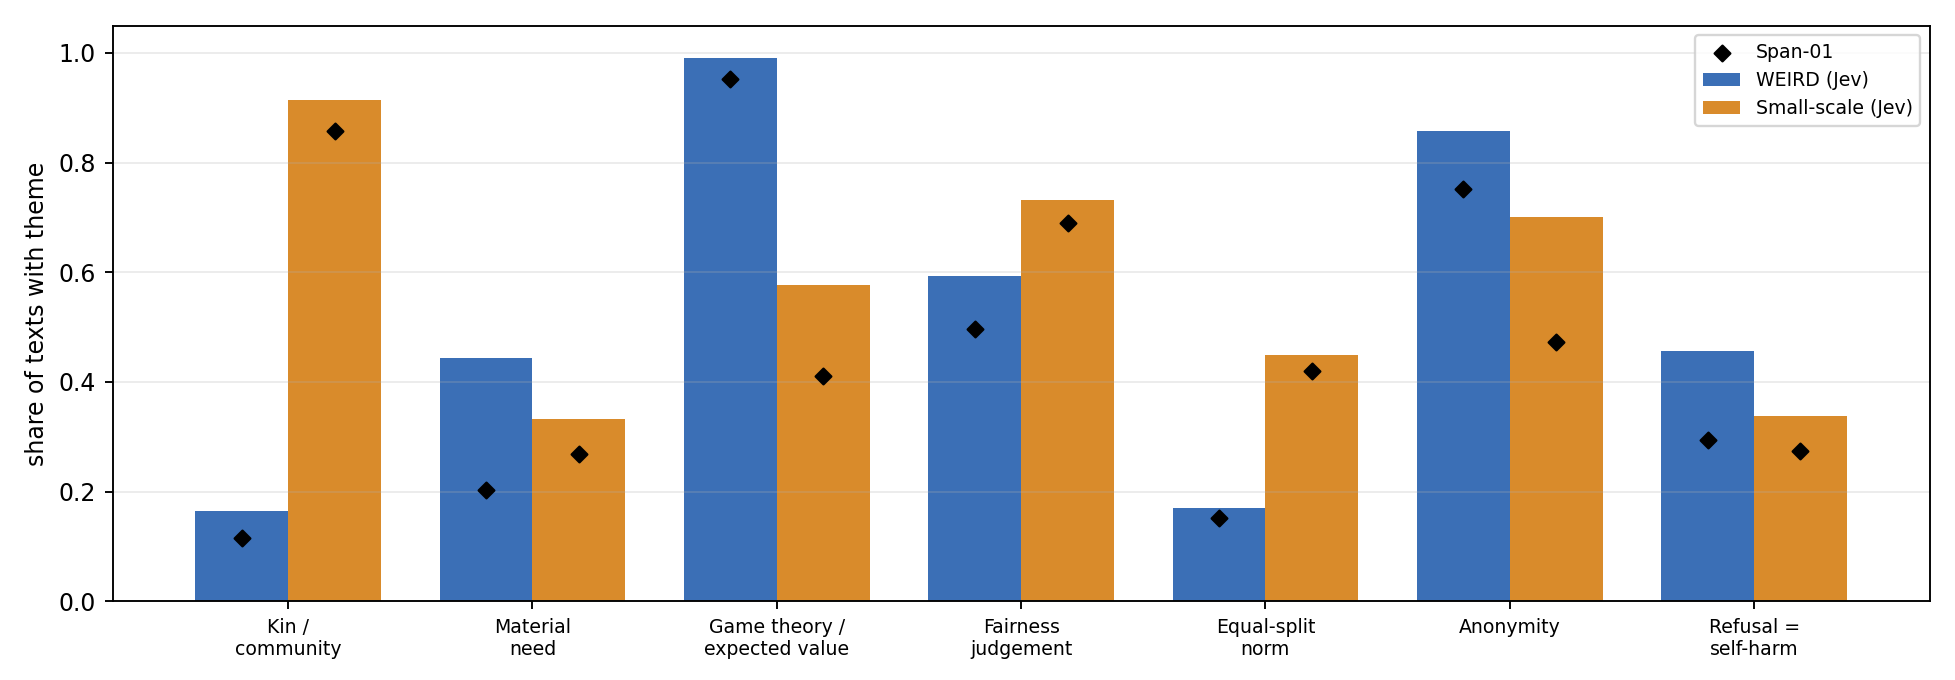
\includegraphics[width=0.98\linewidth]{figs/fig17_themes_s2.png}
\caption{Share of Study~2 responder justifications containing each theme, by arm ($n = 1\,500$). Bars: Jev~1.13; black diamonds: Span-01.}
\label{fig:themes2}
\end{figure}

Unlike Study~1, discourse and decision agree in Study~2. Of justifications ending in rejection, 94--96\% invoke kin/community, nearly all (99.6--100\%) a fairness judgement and 76--81\% an equal-split norm, while only 5--8\% contain expected-value reasoning; 80--92\% of accepting justifications rest on expected-value reasoning. A typical small-scale rejection (Gemma, 10\% offer): \emph{``In my community, we survive through fair sharing and mutual support; taking 90 while leaving me with 10 is an insult to the principle of reciprocity.''} Rejections repeat the card's own phrases (``reciprocity'', ``sharing'', ``community''). The resulting picture is the opposite of Henrich's field data, where societies with low market integration reject low offers \emph{less} often. Whether this reversal comes from the models' own image of the culture or from the card's value-laden words is tested in the next section.


\section{Description test: where does the reversed gap come from?}\label{sec:wording}

\subsection{Design and hypotheses}

The small-scale card of Study~2 is derived from Henrich's ethnographies but contains value-laden phrases: ``buffered by kinship network'', ``dense kin network, daily face-to-face community'', ``non-market reciprocity, sharing, barter''. Telling a model ``you live by reciprocity and sharing'' may directly supply a reason to reject an unfair split. To test this, in a pre-registered test the same identities (age and occupation/livelihood held fixed) were described in three different texts, none with numeric attributes:

\begin{itemize}
\item \textbf{Value-laden description:} the Study~2 card (control).
\item \textbf{Minimal description:} age and occupation/livelihood only (e.g., ``age: 41 / role in life: seasonal labor'').
\item \textbf{Ethnographic description:} age, occupation and three lines stating community size and market integration factually --- the variables that covary with punishment and with fairness, respectively, in the human data \citep{henrich2010markets}. Small-scale cards: ``a settlement of about 80--300 people, several hours' travel from the nearest town''; ``most food comes from your own household's work; money is used a few times a year at a distant market''; ``dealings with people you do not know: rare; most people you deal with you have known all your life''. WEIRD cards: ``a city of about 0.4--3 million people''; ``almost everything is bought with money in shops and online''; ``several money transactions with strangers every day''.
\end{itemize}

The minimal and ethnographic descriptions passed an additional linter banning \emph{share, reciprocity, barter, kin, community, cooperate, trust, fair, generous, solidarity, gift, mutual} and their derivatives. Design: 3 models $\times$ 2 arms $\times$ 2 offers (10\%, 20\%) $\times$ 50 identities $\times$ 3 descriptions; each identity saw all three (1\,800 valid calls). The primary outcome is the small-scale $-$ WEIRD gap at a 10\% offer (three models pooled). Each new description was assigned to one of four pre-defined classes: \emph{reversed gap} (gap $\geq 0.15$, $p_{\text{Bonf}} < 0.01$, $|h| \geq 0.3$), \emph{Henrich-direction gap} (gap $\leq -0.15$, same criteria), \emph{no gap} ($|$gap$| < 0.05$) or \emph{inconclusive}. The overall reading was also fixed in advance: if the reversed gap persisted under both new descriptions, the models' own cultural image would be supported; if it persisted under neither, we would conclude that it comes from the words of the description.

\subsection{Results}

\begin{table}[H]
\centering
\caption{Description test: rejection rate at a 10\% offer (small-scale / WEIRD). Same identities; only the description text changes.}
\label{tab:wording}
\begin{tabular}{lccc}
\toprule
 & Value-laden & Minimal & Ethnographic \\
\midrule
All three models & \textbf{0.61 / 0.07} & 0.21 / 0.24 & 0.13 / 0.09 \\
\quad gap (S $-$ W) & $+0.54$ & $-0.03$ & $+0.05$ \\
\quad class & reversed & no gap & no gap \\
\midrule
Claude Haiku 4.5 & 0.34 / 0.00 & 0.00 / 0.00 & 0.00 / 0.00 \\
Gemma-4-31b-it   & 1.00 / 0.16 & 0.60 / 0.72 & 0.40 / 0.26 \\
GPT-OSS-120b     & 0.48 / 0.04 & 0.02 / 0.00 & 0.00 / 0.00 \\
\bottomrule
\end{tabular}
\end{table}

\begin{figure}[H]
\centering
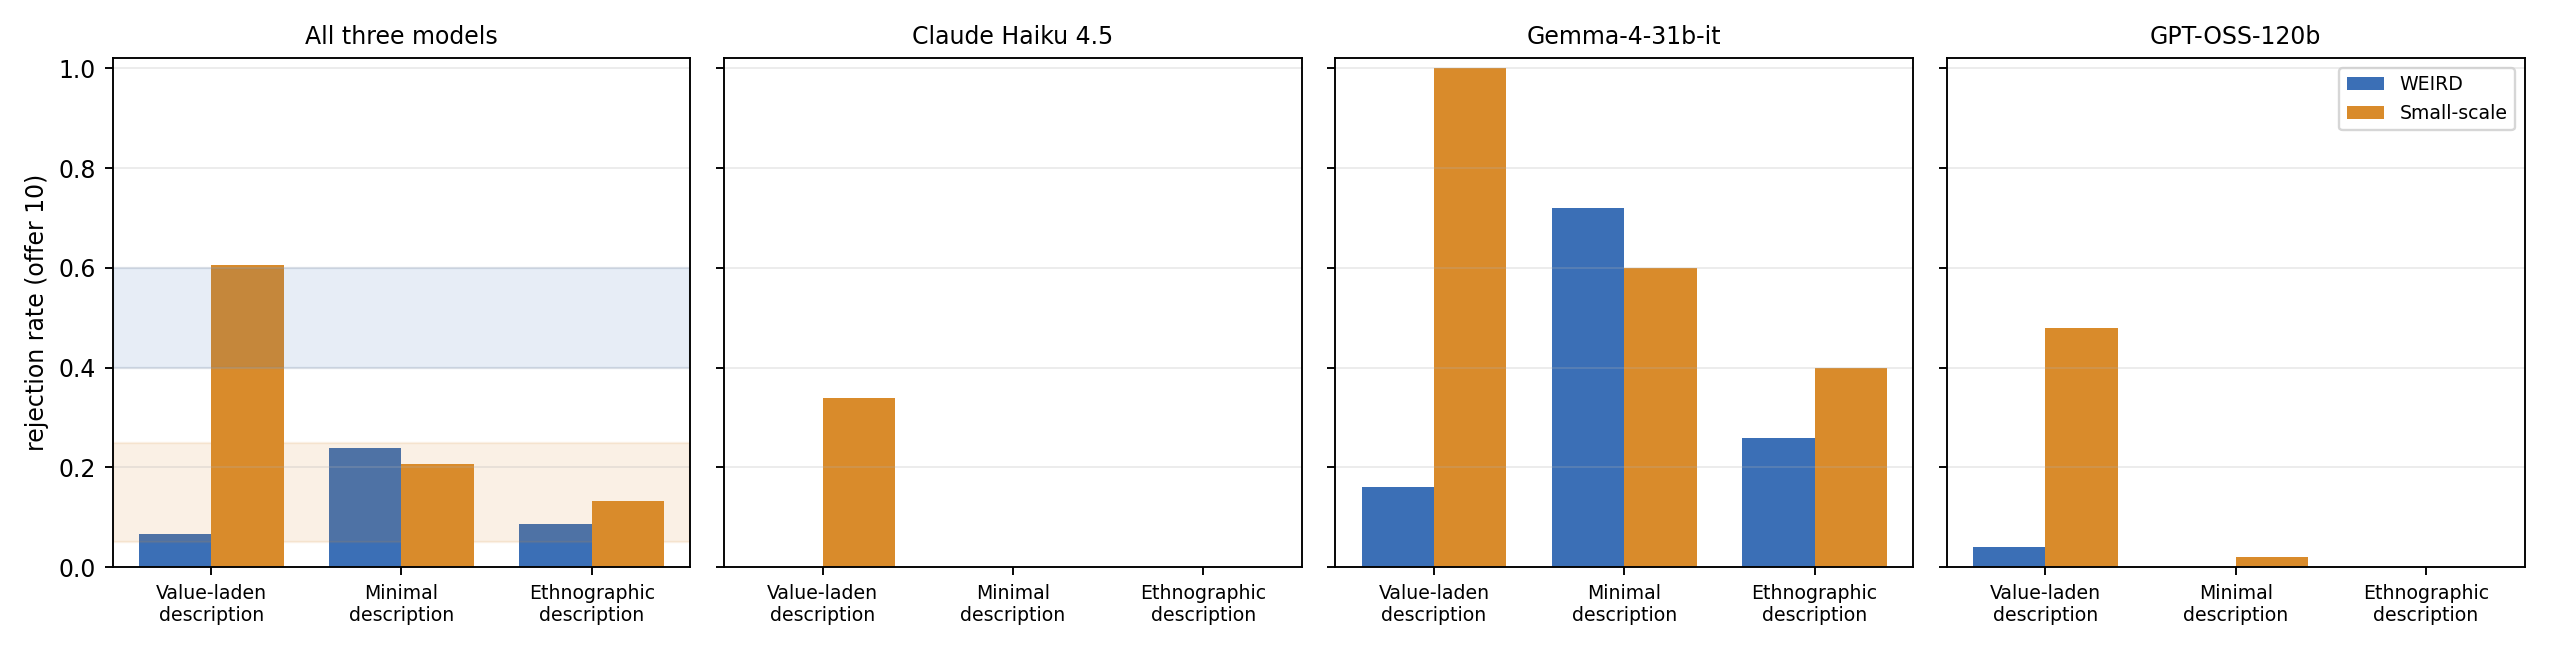
\includegraphics[width=\linewidth]{figs/fig18_wording.png}
\caption{Description test: rejection rate at a 10\% offer. Shaded areas in the left panel are Henrich's human anchors (blue WEIRD, orange small-scale). The reversed gap appears only with the value-laden description; with the minimal and ethnographic descriptions there is no difference between arms, and no description reproduces the human pattern.}
\label{fig:wording}
\end{figure}

The value-laden description replicated Study~2 (small-scale 61\%, WEIRD 7\%). When the same identities were described minimally or ethnographically, the reversed gap vanished: 21\% vs.\ 24\% with the minimal description (gap $-0.03$, $p_{\text{Bonf}} = 0.98$) and 13\% vs.\ 9\% with the ethnographic description (gap $+0.05$, $p_{\text{Bonf}} = 0.39$). Both new descriptions fell into the pre-defined ``no gap'' class; by the pre-specified reading, \textbf{the reversed gap of Study~2 comes from the value-laden words of the description}. At the model level, Haiku and GPT-OSS almost never rejected in either arm under the two new descriptions; Gemma rejected at high rates under both, with inconclusive differences between arms. At a 20\% offer (a pre-specified secondary outcome) the value-laden description again gave a reversed gap (44\% vs.\ 0\%) and the ethnographic description no rejections in either arm. The minimal description gave a small difference in the Henrich direction (small-scale 5\% vs.\ WEIRD 13\%; gap $-0.08$, $\chi^2$ $p = 0.014$; class ``inconclusive''). This difference comes entirely from Gemma (14\% vs.\ 38\% at a 20\% offer, 60\% vs.\ 72\% at 10\%), whose rejection rates in both arms are far above the human small-scale range. No description produced a gap meeting the pre-defined Henrich-direction class, and none reproduced the human pattern of levels.

\verdictbox{DESCRIPTION TEST PRE-REGISTERED DECISION: the reversed gap comes from the words of the description; no description reproduces Henrich's pattern.}

The ethnographic description is especially informative: it gives the model, stated factually, the two variables associated with fairness and punishment in the human data --- market integration and community size \citep{henrich2010markets}. With this information, too, the models did not reproduce the human pattern; identities with low market integration did not reject low offers less often than identities with high market integration. The relationship ``market integration $\to$ fairness norms toward strangers'', which is plausibly present in the models' training data, is not reflected in behavior under this form of description.


\section{General Discussion}

\subsection{The description sets the outcome}

The main finding is that in LLM agents steered by an identity description, the cross-cultural outcome depends more on how the description is written than on the culture being simulated. For the same people, game and offers we obtained three different pictures: with a numeric fairness score in the description, almost no rejection (Study~1); with value-laden phrases such as ``reciprocity, sharing, kin'', a strong reversed gap (Study~2); with a plain or factual description, no gap (Section~\ref{sec:wording}). None of the three resembles Henrich's field data.

The reversed gap under the value-laden description shows how the models read these phrases. The small-scale card's ``non-market reciprocity, sharing, barter'' is an ethnographically accurate description; many of Henrich's societies are characterized by such exchange relationships. The models, however, read it as ``I protect the reciprocity norm by punishing an unfair split'' and repeat the phrases directly in their justifications. The field data show the opposite: reciprocity based on close relationships does not transfer to a one-shot split with an anonymous stranger, and fairness toward strangers increases with market integration, and costly punishment with community size \citep{henrich2001,henrich2010markets}. The models' inference is intuitively plausible but empirically wrong, and it is triggered by the presence of those words in the description. The findings agree with work showing that LLM persona simulations misportray groups \citep{cheng2023compost,wang2025misportray}; here, however, the direction and size of the misportrayal are set less by the model's own image than by the words the researcher chooses.

\subsection{Numeric attributes and value-laden words: two steering channels}

The numeric fairness score and the value-laden words are two forms of the same problem: the description implies, directly or indirectly, the behavioral disposition of the simulated person. Assigning numeric disposition parameters to agents is standard in classical agent-based modeling and was done here in that spirit; in LLM agents, however, such a parameter largely determines the decision even when it is presented with the note ``for your own reflection, not instructions''. Banning the word ``fair'' from the card text while presenting a variable called ``fairness\_salience'' on the same card let the steering out of the door and back in through the window. The same principle applies to value-laden words. The results are consistent with the prompt-sensitivity literature \citep{sclar2024quantifying}; the difference is that the changes here are not meaning-preserving formatting differences but descriptions that each emphasize a different, defensible aspect of the same identity. A researcher could choose any of them in good faith and report one of three very different results.

\subsection{Source of the pot}\label{sec:source}

The two tests in Appendix~\ref{sec:mechanism} point to a second variable affecting rejection. Recognizing the game by name is not necessary for acceptance (Appendix~\ref{sec:disguise}); by contrast, a single sentence stating that the pot was earned by both parties with equal effort raised low-offer rejection from 1.5\% to 13.3\% in the game frame and from 6.2\% to 32.3\% in the story frame (Appendix~\ref{sec:entitle}). The effect also appears with the numbers hidden and is clearly larger than that of a placebo sentence using the same language of effort but decoupling the effort from the pot. It is directionally consistent with entitlement effects in human experiments \citep{hoffman1994,cherry2002,oxoby2008}. It depends strongly on the model: Haiku and Gemma reject at rates reaching the human range, while GPT-OSS does not change. The similarity between models observed in the standard paradigm is therefore paradigm-dependent; the contribution of alignment methods to these differences cannot be determined without comparing base versions of the same models.

\subsection{Implications for GABM practice}

Three practical recommendations follow. First, numeric variables that directly imply a behavioral outcome (fairness, risk attitude, cooperativeness, etc.) should be removed from identity descriptions or their effect measured with a separate manipulation. Second, the value-laden phrases used to describe cultural groups can be the source of the result and should be varied systematically, with results reported under more than one description. Third, a cross-cultural difference obtained under a single description should not be taken as evidence that the difference belongs to the simulated groups; only differences that replicate against human data and independently of the description can be interpreted that way.


\section{Limitations}

\begin{enumerate}
\item \textbf{One paradigm, three models.} All experiments use the Ultimatum Game and three mid-sized model families; the largest frontier models and other behavioral paradigms were not tested.
\item \textbf{Limited description variety.} Only three description texts were tested. Which phrase of the value-laden description (``reciprocity'', ``sharing'', ``kin'') produces the reversed gap was not isolated. Under the minimal description one model (Gemma) rejected somewhat more on WEIRD cards; whether this is a stable property of that model was not tested. All texts are in English.
\item \textbf{Limited within-arm diversity.} Without numbers, cards within an arm differ only in age and occupation/livelihood; 50 cards per cell represent 50 similar descriptions, not 50 independent people. The small-scale arm is a composite of Henrich's ethnographies, not one real society.
\item \textbf{Sequential design.} Each test was designed after seeing the result of the previous one. Each test's plan was written before its own data and post-pilot changes were recorded as dated amendments, but these plans were not uploaded to a public registry, and the order and choice of tests were determined in response to the data. In the numeric-attribute test the identity hypothesis anticipated only the Henrich direction; the reverse-direction gap was reported as a separate note, and both directions were pre-specified in subsequent tests.
\item \textbf{Mechanism tests used numeric cards.} The disguised-game and entitlement tests used Study-1-style cards (Appendix~\ref{sec:mechanism}). The entitlement effect was also observed with numbers hidden; the causal role of game recognition remains open because of the floor effect of numeric cards.
\item \textbf{Coding method.} Clustering of texts sent in one batch to a single LLM was originally planned; because this method can be affected by text order, it was replaced by per-text coding with decision models. The decision-model coders are closed and new; the high agreement between two providers (median Cohen $\kappa = 0.74$) reduces but does not remove this risk.
\item \textbf{Reproducibility of Study~1 cards.} Study~1 card seeds were generated with Python's per-process salted hash function; the cards cannot be regenerated from the seeds, but all cards used are stored. All later experiments use fixed seeds.
\end{enumerate}


\section{Conclusion and Future Work}

Our attempt to reproduce Henrich's cross-cultural Ultimatum finding with LLM agents failed, and the form of the failure was set not by the simulated culture but by how the identity was described. This reframes the question ``Can LLMs simulate human behavior?''. The output of an LLM steered by an identity description is not a measurement of the simulated group's behavior but of how that group was described. Unless cross-cultural GABM studies report results under more than one description and test them against a human anchor, they cannot know whether their findings belong to the simulated culture or to the researcher's words.

Three follow-up questions stand out: (i) which phrase of the value-laden description produces the reversed gap, and does the effect persist in other languages and larger models; (ii) is the same description sensitivity observed in a second behavioral paradigm (e.g., dictator or public-goods games); (iii) do description sensitivity and entitlement sensitivity differ between base and instruction-tuned versions of the same models.


\section*{Data and code availability}

All experiment code, prompts, identity descriptions, pre-registration files (with dated amendments), raw logs of every API call and analysis scripts are in the replication package: \url{https://github.com/gkhngyk/llm-culture-description}. Experiments were run through OpenRouter with the model versions stated; because closed models may be updated on the provider side, exact reproduction cannot be guaranteed. The repository is released under the CC BY 4.0 license.

\section*{AI assistance statement}

The experimental design, coding, analysis and writing of this study were carried out to a large extent together with an AI coding assistant (Anthropic Claude, via Claude Code). All design decisions, interpretations and text were reviewed and approved by the author, who takes responsibility for the content. The models used as experimental subjects and the decision models used to code justifications are described separately in the Method section.

\section*{Competing interests and funding}

The study was funded by Empler AI, an artificial intelligence company of which the author is a partner; funding consisted of API usage fees for the models used in the experiments (via OpenRouter). No grants or support were received from any other organization. Apart from standard API usage fees, the author has no financial relationship with the model providers used in the study (Anthropic, Google, OpenAI, TypeSafe, Respan).


\appendix

\section{Mechanism tests}\label{sec:mechanism}

The two tests in this appendix were designed, before the effect of numeric attributes was discovered, to ask why Study~1 produced almost no rejections, and were run with Study-1-style numeric cards. Their results should be read under this condition; the entitlement effect was also tested with the numbers removed (Section~\ref{sec:numbers}). The main text gives only a summary (Section~\ref{sec:source}).

\subsection{Game recognition in Study 1}

In Study~1, 14.6\% of Haiku justifications named the game (``ultimatum'') even though it appears nowhere in the prompt (Table~\ref{tab:gamerecog}). This could be read as the model recognizing the paradigm and retrieving the textbook answer.

\begin{table}[H]
\centering
\caption{Share of justifications containing ``ultimatum'' and game-theory terms. None of these terms appears in the prompt chain.}
\label{tab:gamerecog}
\begin{tabular}{lrrrr}
\toprule
Model & Role & ``ultimatum'' & GT terms & $n$ \\
\midrule
Claude Haiku 4.5 & responder & \textbf{14.6\%} & \textbf{27.0\%} & 500 \\
Gemma-4-31b-it   & responder & 0.2\%           & 12.8\%          & 500 \\
GPT-OSS-120b     & responder & 0.2\%           & 10.4\%          & 500 \\
\midrule
Claude Haiku 4.5 & proposer  & 26.0\%          & ---             & 500 \\
\midrule
Haiku + role forcing & responder & \textbf{0.0\%} & 5.3\%       & 150 \\
\bottomrule
\end{tabular}
\end{table}

\subsection{Game recognition is not necessary for acceptance: disguised-game test}\label{sec:disguise}

Under the game-recognition hypothesis, LLM responders recognize the paradigm as the ``Ultimatum Game'' and retrieve the textbook answer (``accept any positive offer''). The hypothesis rested on a correlation in Study~1 (Table~\ref{tab:gamerecog}). The disguised-game test examined it by manipulation. The same profiles were compared in three conditions: (i) the original primary prompts (control); (ii) a \emph{wallet} story --- two strangers returned a lost wallet together, the 100-coin reward was given to the other person to divide, and if the share is refused the reward is cancelled; (iii) an \emph{orchard} story --- two strangers gathered 100 fruits from an abandoned orchard, the other person made two piles, and if the division is objected to all fruit is left in the orchard. Both stories preserve the payoff structure (fixed 100, unilateral division, take or refuse only, both receive zero on refusal, no future interaction or identification) and contain none of the paradigm's giveaway words (\textit{experiment, participant, offer, split, pot, accept/decline, one-shot, anonymous, game}), checked by a linter. Design: 3 models $\times$ 2 arms $\times$ 5 offers $\times$ 50 profiles $\times$ 3 conditions (4\,491/4\,500 valid calls). Hypotheses, the decision rule and a design correction noticed in a pilot (refusal must not send the money to a third person) were recorded before the main run.

\begin{table}[H]
\centering
\caption{Disguised-game test: rejection rate at low offers (10\% and 20\%) and share of justifications naming the game ($n \approx 500$ per condition and model).}
\label{tab:disguise}
\begin{tabular}{lrrrrrr}
\toprule
 & \multicolumn{3}{c}{Low-offer rejection} & \multicolumn{3}{c}{Game recognition} \\
Model & Control & Wallet & Orchard & Control & Wallet & Orchard \\
\midrule
Claude Haiku 4.5 & 0.000 & 0.005 & \textbf{0.210} & \textbf{0.156} & 0.012 & 0.016 \\
Gemma-4-31b-it   & 0.015 & 0.005 & 0.035 & 0.000 & 0.000 & 0.000 \\
GPT-OSS-120b     & 0.005 & 0.000 & 0.000 & 0.002 & 0.000 & 0.000 \\
\midrule
Pooled           & 0.007 & 0.003 & 0.082 & & & \\
\bottomrule
\end{tabular}
\end{table}

\begin{figure}[H]
\centering
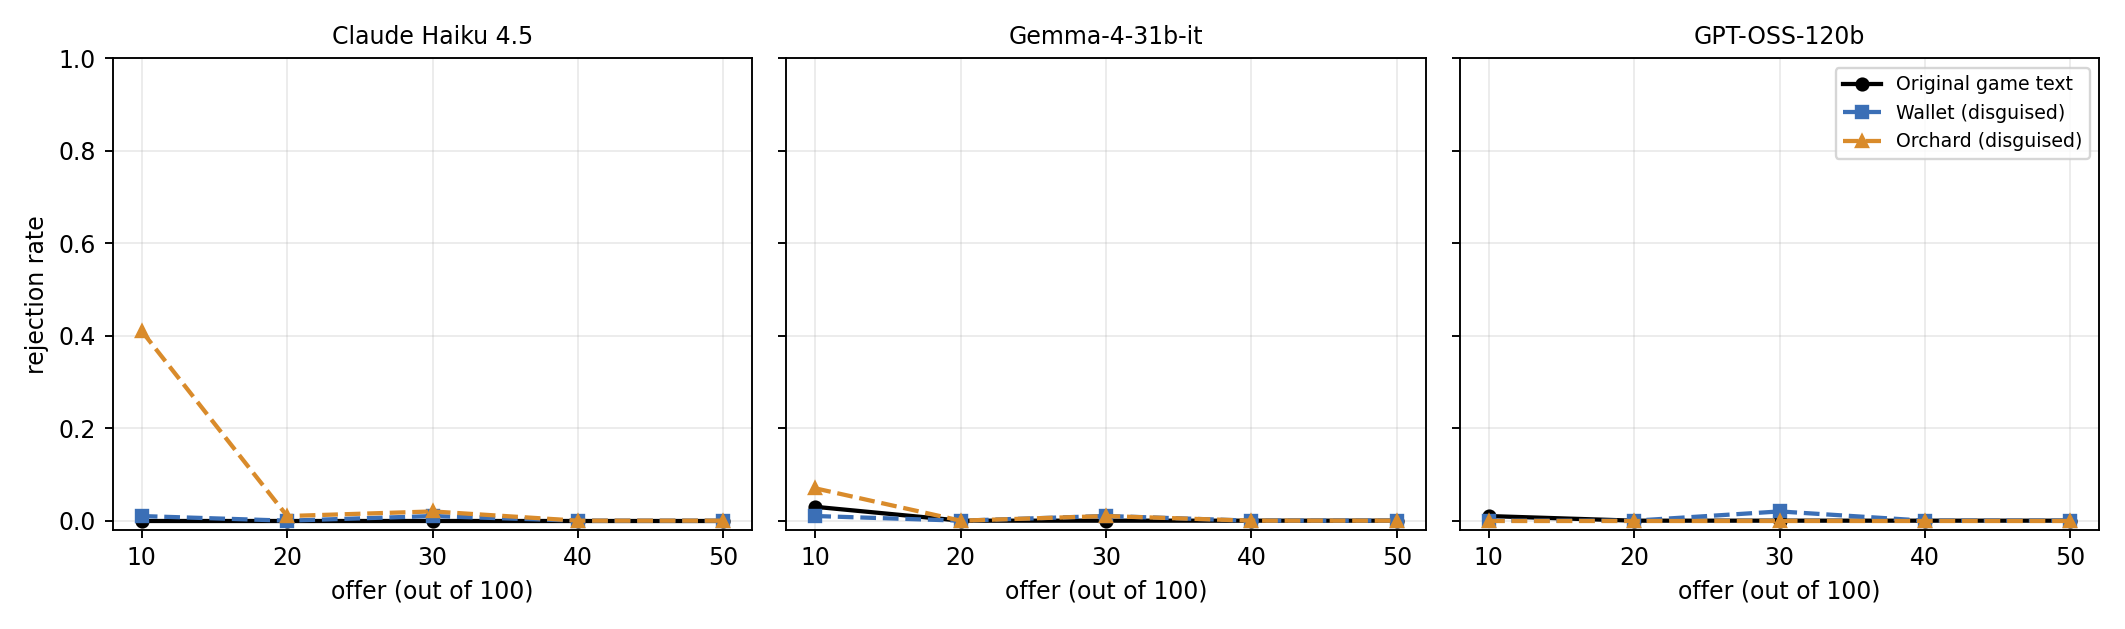
\includegraphics[width=0.98\linewidth]{figs/fig13_disguise.png}
\caption{Disguised-game test: rejection rate by offer (arms pooled). The wallet story does not change acceptance in any model; the orchard story raises low-offer rejection only in Haiku.}
\label{fig:disguise}
\end{figure}

The manipulation worked as intended: Haiku's game-recognition rate dropped from 15.6\% to 1--2\% (Table~\ref{tab:disguise}). In the wallet story, however, rejection did not change (pooled 0.7\% $\to$ 0.3\%; McNemar $p = 0.63$). In the orchard story the pooled rate rose to 8.2\% ($p_{\text{Bonf}} < 10^{-11}$), but almost entirely because of Haiku (0\% $\to$ 21\%). Under the pre-registered decision rule (a rise $\geq 0.10$ in both stories) the result was classified as \textbf{inconclusive / story-dependent}.

The result has two implications. First, in the wallet story recognition disappeared but behavior did not change. This test, however, used numeric cards, which already push rejection to the floor (Section~\ref{sec:numbers}); even if removing recognition raised rejection, the effect could be invisible because of the floor. The numbers-free data do not settle the causal role of recognition either: in the numeric-attribute test the difference between the game text and the disguised story (windfall pot, numbers hidden) goes in opposite directions across models (small-scale rejection rises from 14\% to 100\% in Haiku but falls from 100\% to 39\% in Gemma and from 43\% to 2\% in GPT-OSS), and Haiku's recognition rate is about 16\% in both frames. The defensible conclusion is narrower: recognizing the game is \emph{not necessary} for acceptance. Gemma and GPT-OSS almost never name the game yet accept low offers on WEIRD cards; in Study~2, Haiku's WEIRD cards never reject, whether or not their justification names the game. Second, the source of the orchard increase is clear in the justifications: all 42 of Haiku's low-offer rejections refer to joint effort or equal contribution (``we both contributed to the collection''); no justification without such a reference ends in rejection. The wallet reward, by contrast, is the product of chance rather than effort. This \emph{exploratory} observation generated the hypothesis that the source of the pot, not the identity of the game, drives over-acceptance, which was tested prospectively in the entitlement test.

\subsection{Source of the pot: entitlement test}\label{sec:entitle}

The entitlement test is a pre-registered $2 \times 2$ experiment that manipulates the source of the pot directly. The first factor is the \emph{frame}: the original game text or the orchard story. The second is the \emph{source}: the pot is a windfall (game text unchanged; in the story, ``came across 100 fruits that had already been picked and left in baskets at the edge of an abandoned orchard'') or was earned by both parties with equal effort. In the game frame the earned condition is a single sentence added to the original text:

\begin{quote}
\itshape
``The 100 units were earned by the two of you together: earlier in the session you both worked on the same task, and each of you did about half of the work.''
\end{quote}

In the story frame only the source sentence changes (``spent the day picking fruit together and collected 100 fruits; each of you did about half of the picking''). Within each frame, windfall and earned conditions thus differ by a single sentence. Design: 3 models $\times$ 2 arms $\times$ 5 offers $\times$ 50 profiles $\times$ 4 cells, each profile seeing all four cells (5\,998/6\,000 valid calls). The pre-registered primary contrasts are the earned $-$ windfall difference in low-offer rejection within each frame (paired exact McNemar, Bonferroni-corrected). Because the effect had appeared in only one model in the exploratory data, the support threshold was set at a rise $\geq 0.05$ in both frames with $p_{\text{Bonf}} < 0.01$.

\begin{table}[H]
\centering
\caption{Entitlement test: rejection rate at low offers (10\% and 20\%); 10\% offer only in parentheses. W = windfall, E = jointly earned.}
\label{tab:entitlement}
\begin{tabular}{lrrrr}
\toprule
 & \multicolumn{2}{c}{Game frame} & \multicolumn{2}{c}{Story frame} \\
Model & W & E & W & E \\
\midrule
Claude Haiku 4.5 & 0.000 (0.00) & 0.060 (0.11) & 0.135 (0.23) & \textbf{0.710 (0.97)} \\
Gemma-4-31b-it   & 0.030 (0.04) & \textbf{0.320 (0.54)} & 0.040 (0.04) & 0.235 (0.27) \\
GPT-OSS-120b     & 0.015 (0.01) & 0.020 (0.02) & 0.010 (0.01) & 0.020 (0.02) \\
\midrule
Pooled           & 0.015 & 0.133 & 0.062 & 0.323 \\
\bottomrule
\end{tabular}
\end{table}

\begin{figure}[H]
\centering
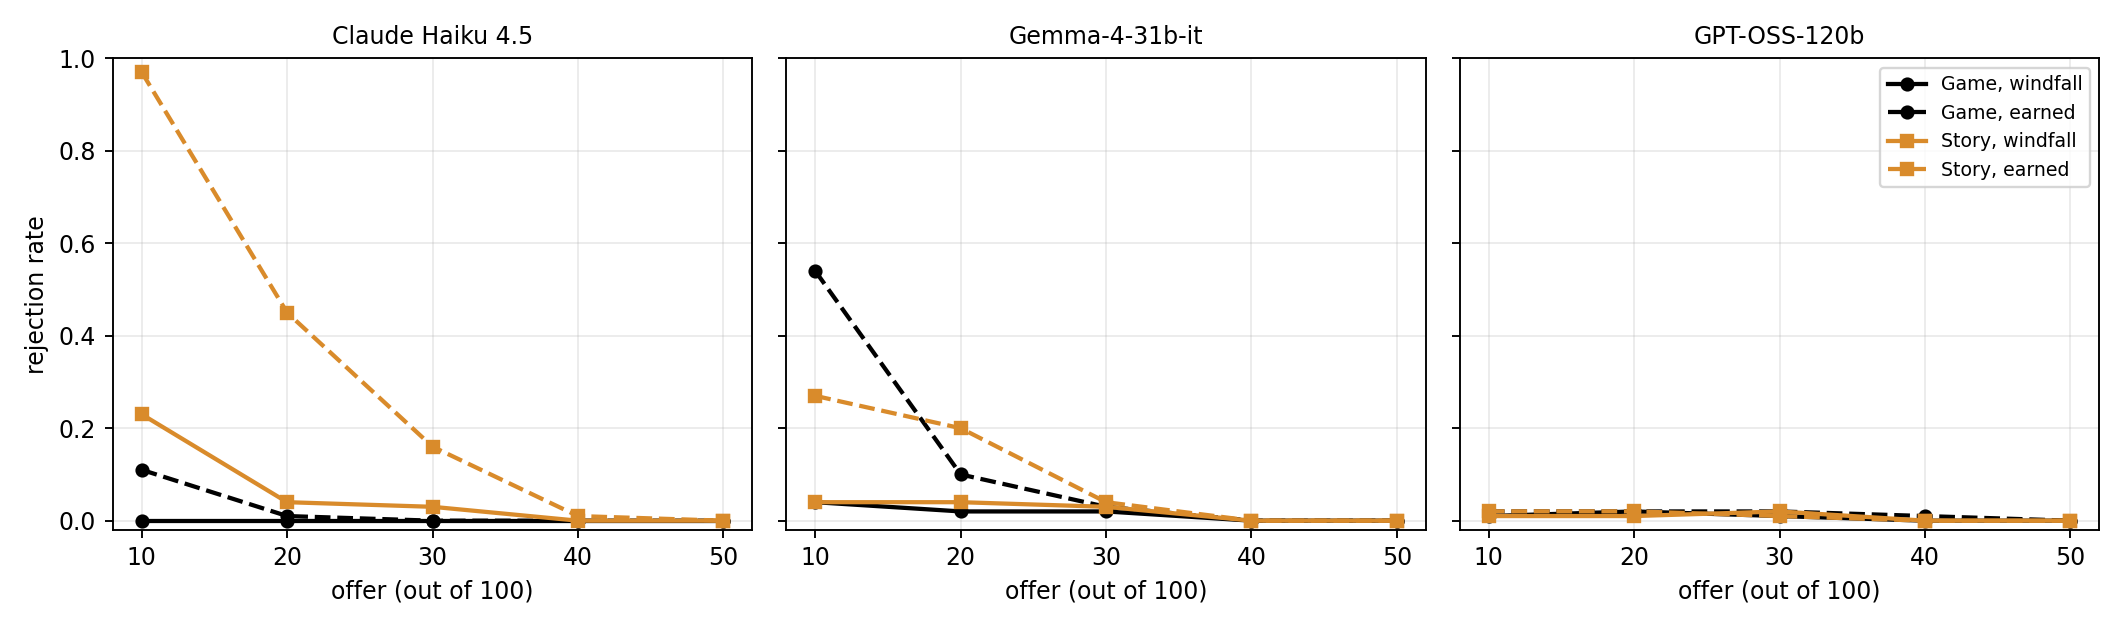
\includegraphics[width=0.98\linewidth]{figs/fig14_entitlement.png}
\caption{Entitlement test: rejection rate by offer (arms pooled). Dashed lines are conditions in which the pot was earned jointly. In Haiku and Gemma a single sentence about effort sharply raises low-offer rejection; GPT-OSS does not change.}
\label{fig:entitlement}
\end{figure}

\textbf{The pre-registered hypothesis is supported.} Stating that the pot was earned jointly raised low-offer rejection from 1.5\% to 13.3\% in the game frame ($+0.118$; 73 profiles switched from accept to reject, 2 in the other direction; $p_{\text{Bonf}} < 10^{-18}$) and from 6.2\% to 32.3\% in the story frame ($+0.261$; 158 vs.\ 2; $p_{\text{Bonf}} < 10^{-43}$). The effect declines monotonically with the offer and disappears at 40--50\% offers; the models reject splits disproportionate to effort, not any split (Figure~\ref{fig:entitlement}).

The effect depends strongly on the model. With an earned pot, Haiku rejects a 10\% offer 97\% of the time in the story frame, having never rejected it in the standard paradigm. In Gemma, effort information raises rejection of a 10\% offer from 4\% to 54\% even within the original game text, inside Henrich's WEIRD range (40--60\%). GPT-OSS stays at about 2\% in all four cells. A manipulation check shows that GPT-OSS noticed the effort information: in the story frame 48.6\% of its justifications in the earned condition mention effort, versus 0.2\% in the windfall condition; in the game frame the difference is 0.17, just below the pre-registered threshold of 0.20. GPT-OSS's insensitivity is thus not due to missing the information but to a decision rule that does not respond to effort.

Secondary analyses show two further patterns. (i) Frame and source interact: the effort effect is larger in the story frame than in the game frame (interaction $+0.143$). (ii) With a windfall pot the frame itself matters only for Haiku (0\% $\to$ 13.5\%; not significant for Gemma and GPT-OSS). Together with the wallet result, this suggests that disguise matters to the extent that the disguised scene implies a joint activity (``fruit we found together''), not by itself.

The pattern is directionally consistent with entitlement effects in human experiments \citep{hoffman1994,cherry2002,oxoby2008}: a responder who shared the effort rejecting a disproportionate split is the responder-side counterpart of the same property-rights logic. The comparison is only directional; no quantitative calibration against human data in the same design was done.

In the numeric-attribute test (Section~\ref{sec:numbers}) the entitlement effect was also compared with a pre-registered placebo. The placebo sentence uses the same language of effort but states explicitly that the effort has nothing to do with the pot (``that practice task was unpaid and had nothing to do with this money''). In Haiku and Gemma the earned pot produced clearly more rejection than the placebo ($+0.175$; McNemar $p < 10^{-100}$), so the effect is not merely a response to the words ``work'' or ``half''. The placebo also raised rejection somewhat relative to the windfall pot ($+0.081$), so the pre-written criterion ($< 0.05$) was not met. The justifications suggest that shared effort unrelated to the pot also creates an expectation of reciprocity (``we did equal work yesterday'').


\bibliographystyle{plainnat}
\bibliography{references}

\end{document}
